\documentclass{bmcart}

%%%%%%%%%%%%%%%%%%%%%%%%%%%%%%%%%%%%%%%%%%%%%%
%%                                          %%
%% CARGA DE PAQUETES DE LATEX               %%
%%                                          %%
%%%%%%%%%%%%%%%%%%%%%%%%%%%%%%%%%%%%%%%%%%%%%%

%%% Load packages
\usepackage{amsthm,amsmath}
\usepackage{graphicx}
%\RequirePackage[numbers]{natbib}
%\RequirePackage{hyperref}
\usepackage[utf8]{inputenc} %unicode support
\usepackage{float}
\usepackage{listings}
\lstset{ %
	language=R,                     % the language of the code
	basicstyle=\footnotesize,       % the size of the fonts that are used for the code
	numbers=left,                   % where to put the line-numbers
	numberstyle=\tiny\color{gray},  % the style that is used for the line-numbers
	stepnumber=1,                   % the step between two line-numbers. If it's 1, each line
	% will be numbered
	numbersep=5pt,                  % how far the line-numbers are from the code
	backgroundcolor=\color{white},  % choose the background color. You must add \usepackage{color}
	showspaces=false,               % show spaces adding particular underscores
	showstringspaces=false,         % underline spaces within strings
	showtabs=false,                 % show tabs within strings adding particular underscores
	frame=single,                   % adds a frame around the code
	rulecolor=\color{black},        % if not set, the frame-color may be changed on line-breaks within not-black text (e.g. commens (green here))
	tabsize=2,                      % sets default tabsize to 2 spaces
	captionpos=b,                   % sets the caption-position to bottom
	breaklines=true,                % sets automatic line breaking
	breakatwhitespace=false,        % sets if automatic breaks should only happen at whitespace
	escapeinside={\%*}{*)},         % if you want to add a comment within your code
} 
%\usepackage[applemac]{inputenc} %applemac support if unicode package fails
%\usepackage[latin1]{inputenc} %UNIX support if unicode package fails


%%%%%%%%%%%%%%%%%%%%%%%%%%%%%%%%%%%%%%%%%%%%%%
%%                                          %%
%% COMIENZO DEL DOCUMENTO                   %%
%%                                          %%
%%%%%%%%%%%%%%%%%%%%%%%%%%%%%%%%%%%%%%%%%%%%%%

\begin{document}

	\begin{frontmatter}
	
		\begin{fmbox}
			\dochead{Research}
						
			\title{Red de los targets de SARS-CoV2}
			
			\author[
			  addressref={aff1},
			  corref={aff1},
			  email={ireero99@uma.es}
			]{\inits{I.R.G}\fnm{Irene} \snm{Romero Granados}}
			\author[
			  addressref={aff1},
			  corref={aff1},
			  email={paulandujar@uma.es}
			]{\inits{P.A.Z}\fnm{Paula} \snm{Andújar Zambrano}}
			\author[
			  addressref={aff1},
			  corref={aff1},
			  email={0619884107@uma.es}
			]{\inits{R.G.M}\fnm{Rosario} \snm{García Morales}}
			\author[
			  addressref={aff1},
			  corref={aff1},
			  email={delcastillosoledad@uma.es}
			]{\inits{S.dC.C}\fnm{Soledad} \snm{del Castillo Carrera}}
			
			
			\address[id=aff1]{%                           % unique id
			  \ordiv{ETSI Informática},             % department, if any
			  \orgname{Universidad de Málaga},          % university, etc
			  \city{Málaga},                              % city
			  \cny{España}                                    % country
			}
		
		\end{fmbox}

		
		\begin{abstractbox}
		
			\begin{abstract} % abstract
			Este proyecto pretende estudiar las interacciones que se producen entre las 29 proteínas del virus SARS-COV-2 y el interactoma humano. Para ello, se recopilarán los datos de interacción comentados, con los que se procederá a realizar un análisis sobre ellos y construir la red de proteínas que conforman los objetivos principales para el virus. En cuanto a las herramientas que se utilizarán, serán la base de datos biológica UniProt para la obtención de los datos de entrada, y el lenguaje de R para los métodos de análisis.
			
			\end{abstract}
			
			%%%%%%%%%%%%%%%%%%%%%%%%%%%%%%%%%%%%%%%%%%%%%%
			%% PALABRAS CLAVE DEL PROYECTO              %%
			%%%%%%%%%%%%%%%%%%%%%%%%%%%%%%%%%%%%%%%%%%%%%%
			
			\begin{keyword}
			\kwd{SARS-COV-2}
			\kwd{interactoma}
			\kwd{R}
			\end{keyword}
		
		
		\end{abstractbox}
	
	\end{frontmatter}
	
	
	%%%%%%%%%%%%%%%%%%%%%%%%%%%%%%%%%
	%% COMIENZO DEL DOCUMENTO REAL %%
	%%%%%%%%%%%%%%%%%%%%%%%%%%%%%%%%%
	
	\section{Introducción}
La familia de los coronavirus son virus infecciosos a los que se llama así debido a que en su superficie tienen puntas en forma de corona. A esta familia se les unió en 2019 el conocido SARS-CoV-2, que ha dado lugar al coronavirus 2 o COVID-19. Esta enfermedad es una enfermedad infecciosa que afecta a las vías respiratorias, de manera leve a moderada. Sin embargo esta enfermedad en personas mayores o con patologías previas puede hacer que se desarrolle la enfermedad con consecuencias o síntomas más graves, pudiendo producir hasta la muerte.

El coronavirus actualmente es considerado un problema de salud global, ya que debido a esta pandemia se han contagiado hasta ahora unas 369.955.862 personas y han fallecido un total de 5.650.738 personas. 

Es por esto que es esencial el estudio de este virus, tanto de sus genes, sus proteínas o como interacciona con el ser humano. 

A día de hoy tras toda la inversión mundial que se ha hecho para poder poner fin a este virus, se sabe que el SARS-CoV-2 está formado por 29 proteínas que interactúan con las células del ser humano pudiendo producir síntomas respiratorios graves hasta poder causar la muerte. A estas interacciones moleculares binarias proteína-proteína se les llama interactoma. 

El interactoma sirve como de punto de partida para estudiar los posibles fármacos que podrían bloquear dichas interacciones y así evitar que el virus entre a la célula y se replique. Gracias al estudio del interactoma ha sido posible la realización de vacunas contra el COVID-19. 

En este proyecto vamos a crear y estudiar la red de interacciones de las proteínas del SARS-CoV-2 con las proteínas humanas, y así poder obtener cuales son las principales funciones biológicas humanas en las que este virus interviene y relacionarlo con la realidad. Todos los recursos usados para la obtención de dicha información la podremos encontrar en el GitHub proporcionado. 



	\section{Materiales y métodos}
\subsection{Carga de librerías y datos}
Para poder llevar a cabo este trabajo, el primer paso a realizar es la carga de librerías necesarias y la carga de datos. Antes de cargar los datos, estos han sido descargados de Uniprot (https://www.uniprot.org/) en formato .csv para poder llevar a cabo el análisis de la red.
Una vez ha sido añadido este fichero al directorio correspondiente (data), se procederá a la carga de librerías.
Las librerías que han sido utilizadas en este proyecto son las siguientes:
\begin{itemsize}
	\item igraph: Esta librería permite realizar análisis de redes, por lo cual, proporciona funciones para manipular gráficos con facilidad.
	\item dplyr: Esta librería proporciona métodos para poder manejar los ficheros de datos.
	\item ggplot2: Esta librería es un paquete de visualización de datos.
	\item zoo: Esta librería está especialmente dirigida a series temporales irregulares de vectores/matrices y factores numéricos. 
	\item STRINGdb: Este paquete proporciona una interfaz para la base de datos STRING de interacciones proteína-proteína.
\end{itemsize}

Después de tener las librerías necesarias y saber la funcionalidad de cada una de ellas, se procederá a cargar el archivo en una variable llamada "data" mediante el método "read.csv()"

Seguidamente, se filtrarán las entradas utilizando el paquete "dplyr" en las que la columna Entry.Name contenga en su nombre "HUMAN" ya que estos son los datos que interesan en esta práctica.

\subsection{Mapeo y primera capa de la red}
A continuación, utilizando la librería STRINGdb, se realiza un mapeo con los datos ya filtrados. Se guardará los hits de string en una imagen png en el directorio de los resultados (results)

Seguidamente, se creará la primera capa de la red y se guardará el resultado de esta primera capa en una imagen png. 

\subsection{Clustering y Linked Communities}
Una vez se tiene los datos ya mapeados y filtrados, se pasa a realizar el clustering. El clustering consiste en agrupar los ítemns en grupos con características similares y así, determinar patrones.
Utilizando el paquete STRINGdb, los datos mapeados han sido clasificados en cuatro grupos diferentes según sus características.

Seguidamente, utilizando el paquete linkcommm, se ha realizado la búsqueda de comunidades. Linkcomm proporciona las herramientas necesarias para generar, visualizar y analizar comunidades dentro de un grafo.

Al obtener las comunidades vinculadas, estas serán guardadas en la carpeta de results y, además, se han obtenido los tamaños de los clusters y han sido clasificados por comunidad/modularidad para así obtener los 6 mejores.

\subsection{Enriquecimiento Funcional}
Al realizar el clustering y el agrupamiento de estas comunidades, se realizará el enriquecimiento funcional. Este enriquecimiento es utilizado para obtener los procesos biológicos de los grupos que han sido formados en el clustering.
En primer lugar, ha sido diseñado el enriquecimiento mediante STRINGdb. Después, se ha realizado el enriquecimiento con GO, es decir, con una ontología génica y también, se ha realizado el enriquecimiento con la ontología KEGG. 

El enriquecimiento ha sido utilizado con los clusters de mayor tamaño y de mayor modularidad.

\subsection{Robustez}
Por último, utilizando los métodos proporcionados en el campus virtual, se ha calculado la robustez de la red de genes. Esta funciona para conocer si la red que se está estudiando es un sistema fuerte y esta no tiende a tener errores. Además, ha sido calculada frente a ataques aleatorios como a ataques dirigidos, pero también, han sido combinados ambos ataques.

 
	\section{Resultados}

\subsection{Red de interacciones y robustez}

La siguiente imagen muestra la red de interaciones del ser humano con las proteínas del SARS-CoV. Como podemos ver el SARS-CoV interacciona con 89 proteínas humanas, produciendo un total de 475 interacciones. 
\begin{figure}
	\centering
	
	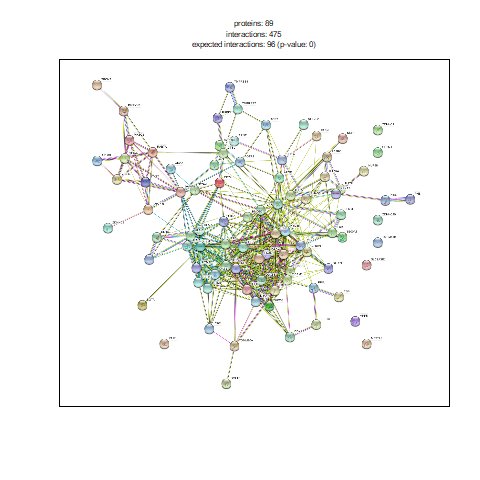
\includegraphics[width=70mm,scale=1.2]{figures/string_hits.png}
	
	\caption{\textit{Red de interacciones del SARS-CoV con las proteínas humanas}}
	
\end{figure}

Tras eliminar los nodos que no están conectados, hemos obtenido la red real de interacciones que podemos ver a continuación. Sin embargo hay demasiadas conexiones como para poder distinguir los nodos. Es por ello que realizaremos los pasos siguientes de clustering, para así poder extraer la información relevante de la red. 
\begin{figure}
	\centering
	
	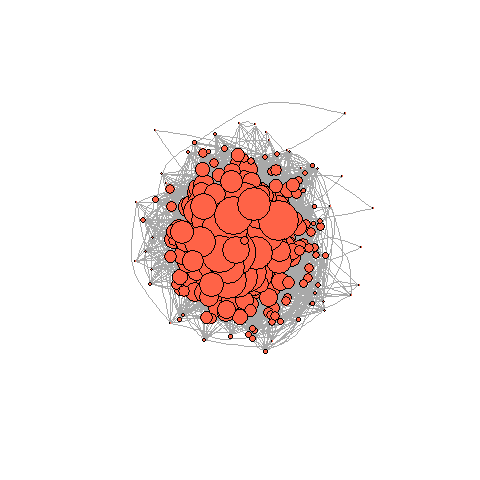
\includegraphics[width=70mm,scale=1.2]{figures/hits.network_graph.png}
	
	\caption{\textit{Red de interacciones del SARS-CoV con las proteínas humanas tras un proceso de filtrado}}
	
\end{figure}


Antes de empezar con ese proceso vamos a estudiar diferentes aspectos de nuestra red. En primer lugar si observamos la imagen, vemos que el la distribución de grado sigue la ley de potencias, por lo tanto nuestra red sigue un modelo de free-scale, lo cual era predecible al estar tratando con una red real. 

Podemos  ver una gran cantidad de hubs. 
\begin{figure}
	\centering
	
	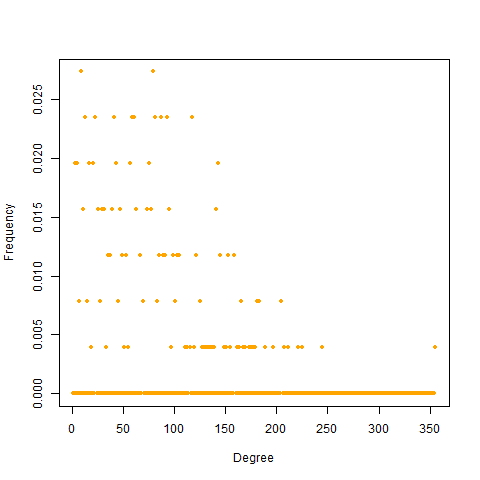
\includegraphics[width=70mm,scale=1.2]{figures/degree_distribution.png}
	
	\caption{\textit{Distribución de grado}}
	
\end{figure}

El coeficiente medio de agrupamiento es de 0.605, lo cual es bastante alto. Además se puede observar la característica propia de las redes reales la cual afirma que conforme el grado de los nodos aumenta, el coeficiente de agrupamiento disminuye. 

\begin{figure}
	\centering
	
	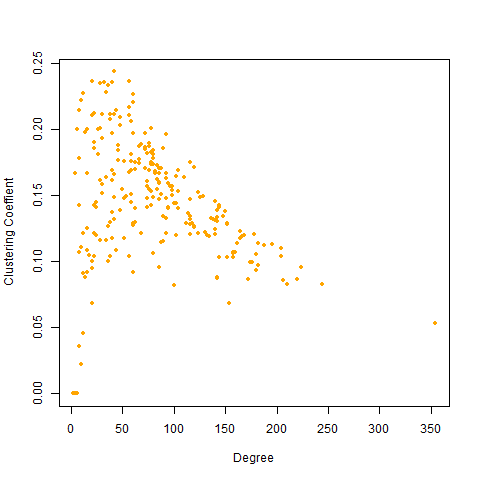
\includegraphics[width=70mm,scale=1.2]{figures/coeficiente_agrupamiento.png}
	
	\caption{\textit{Coeficiente de Agrupamiento}}
	
\end{figure}


La distancia media entre nodos es de 2.03, una medida muy pequeña que puede significar que los nodos tienen un alto índice de conexiones. Esta medida es la que le da la propiedad de mundo pequeño, es decir, la distancia entre nodos elegidos al azar en una red es muy pequeña. 
\begin{figure}
	\centering
	
	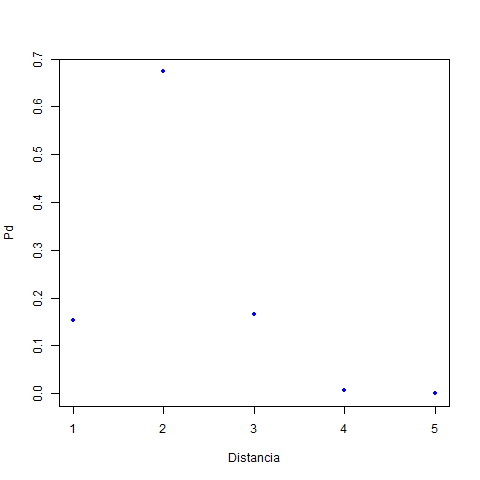
\includegraphics[width=70mm,scale=1.2]{figures/distancia.png}
	
	\caption{\textit{Distancia entre nodos}}
	
\end{figure}

Por último vamos a estudiar la robustez de nuestra red. Para poder estudiar cual es la capacidad de nuestra red de mantener sus funciones frente a la presencia de "ataques" y ver cuán de adaptable es, usamos la robustez. Podemos observar que para ataques aleatorios es bastante robusta, mientras que para ataques dirigidos es más débil. Pues a que tenemos una red real, estos resultados resultan obvios, ya que es más fácil destruir una red si atacas a puntos estratégicos como son los hubs, dónde el tamaño de la componente conexa se reduce drásticamente cuando eliminamos una pequeña fracción de los nodos (hubs). 

\begin{figure}
	\centering
	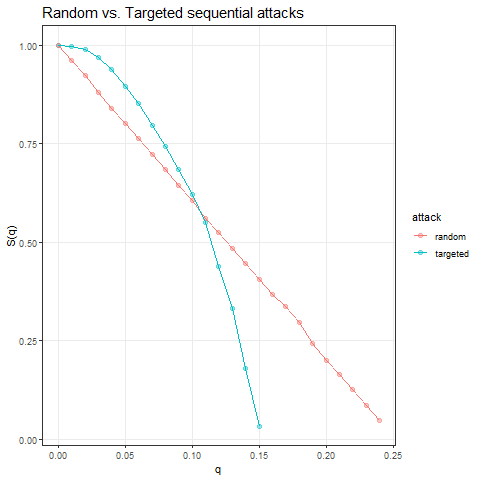
\includegraphics[width=70mm,scale=1.2]{figures/sequential_attacks.png}
	\caption{\textit{Robustez frente a ataques dirigidos y aleatorios}}
\end{figure}

\subsection{Linked Communities}
En esta sección se explicarán los resultados obtenidos aplicar los métodos de comunidades enlazadas a nuestra red, para los cuales hemos usado el paquete linkcomm.

Para ello, primero hemos obtenido estas comunidades aplicando un 'single clustering'. Se ha guardado una imagen del resumen de estas comunidades para un resultado más visual.

\begin{figure}
	\centering
	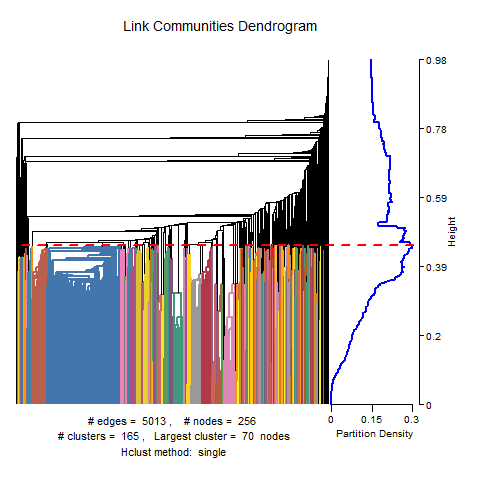
\includegraphics[width=70mm,scale=1.2]{figures/covid_lc_summary.png}
	\caption{\textit{Esquema de las comunidades obtenidas}}
\end{figure}

Podemos observar que este método ha definido 165 comunidades diferentes, la mayor de estas tiene 70 nodos lo cual podemos deducir que hay varias comunidades que comparten nodos.

Para poder analizar un poco las comunidades las hemos filtrado por tamaño y modularidad. Las gráficas generadas para este propósito las mostramos a continuación.

\begin{figure}
	\centering
	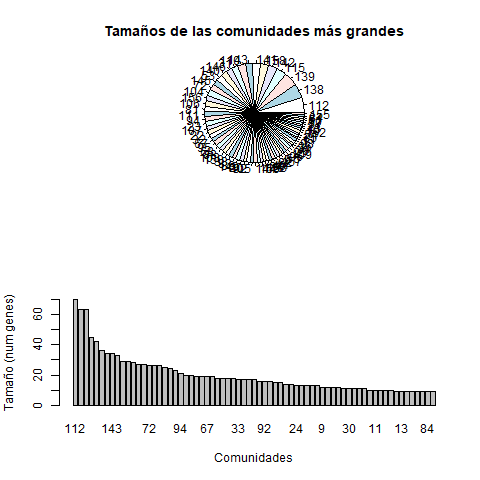
\includegraphics[width=70mm,scale=1.2]{figures/lc_larger_clusters.png}
	\caption{\textit{Comunidades por tamaño}}
\end{figure}

\begin{figure}
	\centering
	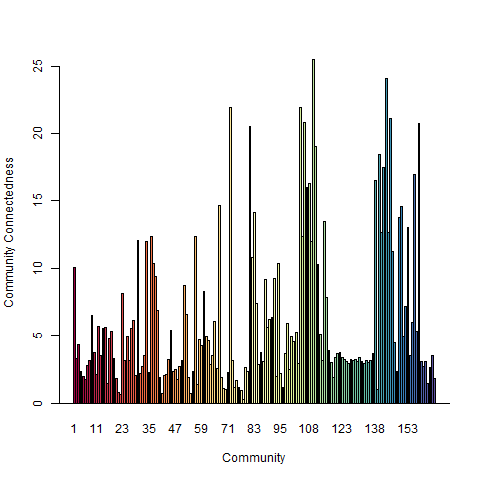
\includegraphics[width=70mm,scale=1.2]{figures/clusters_modularity.png}
	\caption{\textit{Comunidades por modularidad}}
\end{figure}

De estas gráficas hemos podido extraer la comunidad 112 siendo esta la más grande y las comunidades 78 y 22 con una mayor modularidad. Estas comunidades serán utilizadas posteriormente para un análisis funcional.

Para una mejor visualización de los resultados, se ha cambiado el diseño de la gráfica al de Fruchterman Reingold, mostrando solo nodos que pertenezcan a 10 o más comunidades.

\begin{figure}
	\centering
	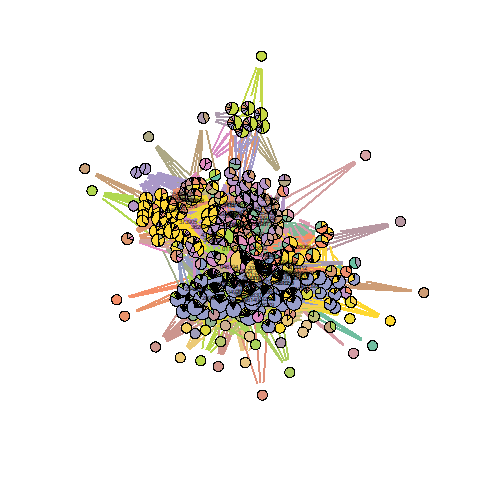
\includegraphics[width=70mm,scale=1.2]{figures/hits.network_layout_fruchterman.reingold_shownodesin_10.png}
	\caption{\textit{Fruchterman Reingold graph}}
\end{figure}

Por otra parte, se han obtenido las comunidades anidadas y se han filtrado para que se muestren las que son independientes de las demás.

\begin{figure}
	\centering
	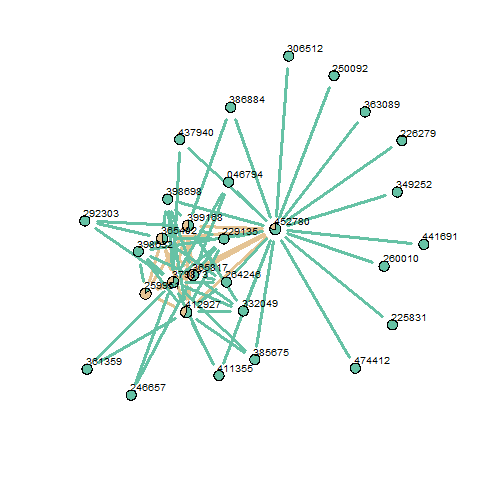
\includegraphics[width=70mm,scale=1.2]{figures/nested_comm.png}
	\caption{\textit{Comunidades anidadas}}
\end{figure}

\subsection{Enriquecimiento funcional}

En esta sección se van a mostrar los resultados obtenidos al realizar el enriquecimiento funcional con GO y con KEGG, mediante el uso de STRINGdb, para los clústeres elegidos.
Se ha guardado la información del enriquecimiento en archivos de tipo csv, y se va a mostrar una imagen de los mismos.

\subsubsection{Clúster 112}

\paragraph{Enriquecimiento con GO}

\begin{figure}
	\centering
	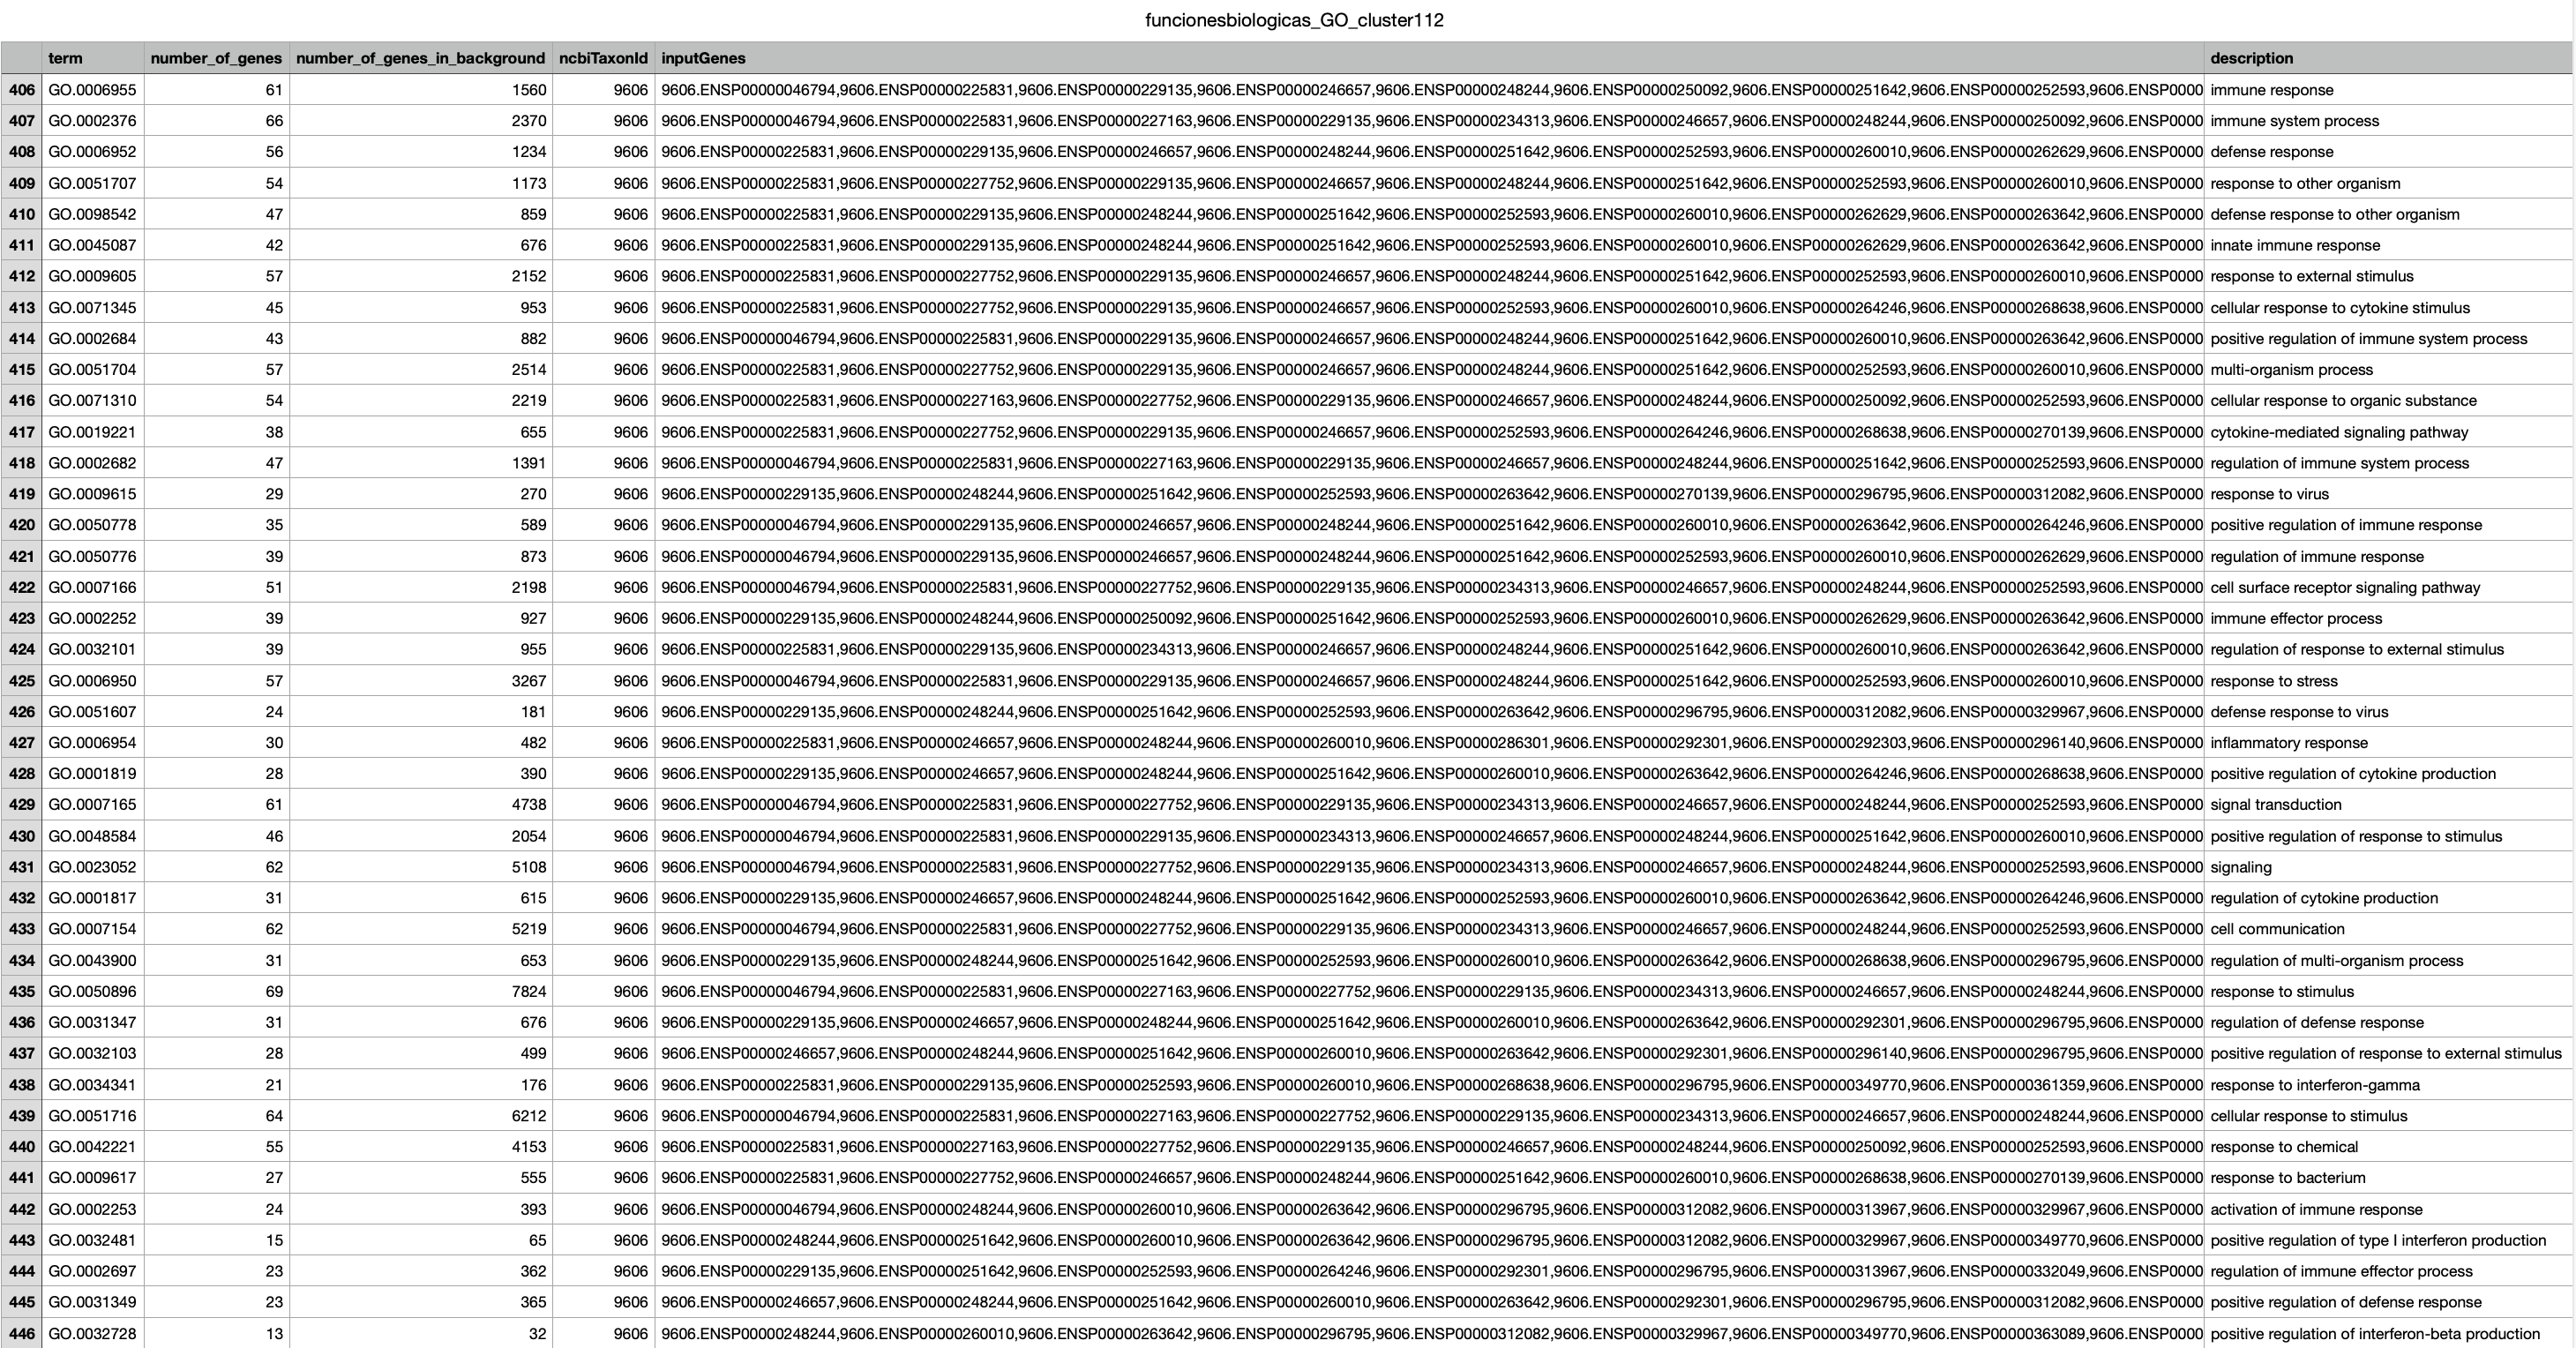
\includegraphics[width=70mm,scale=1.2]{figures/cluster112_GO.png}
	\caption{\textit{Funciones biológicas clúster 112 con GO}}
\end{figure}

Se puede observar que las funciones biológicas visibles están relacionadas con la defensa del organismo, por lo que se puede deducir que son proteínas que forman parte del sistema inmunológico de nuestro organismo. No obstante, en la imagen solo aparecen algunas funciones biológicas. Si se sigue observando el archivo generado nos encontramos con:

\begin{figure}
	\centering
	
\includegraphics[width=70mm,scale=1.2]{figures/cluster112_GO_2.png}
	\caption{\textit{Funciones biológicas clúster 112 con GO}}
\end{figure}

Aquí observamos que otras tantas funciones biológicas están asociadas con la regulación de diversos procesos biológicos.

\paragraph{Enriquecimiento con KEGG}

\begin{figure}
	\centering
	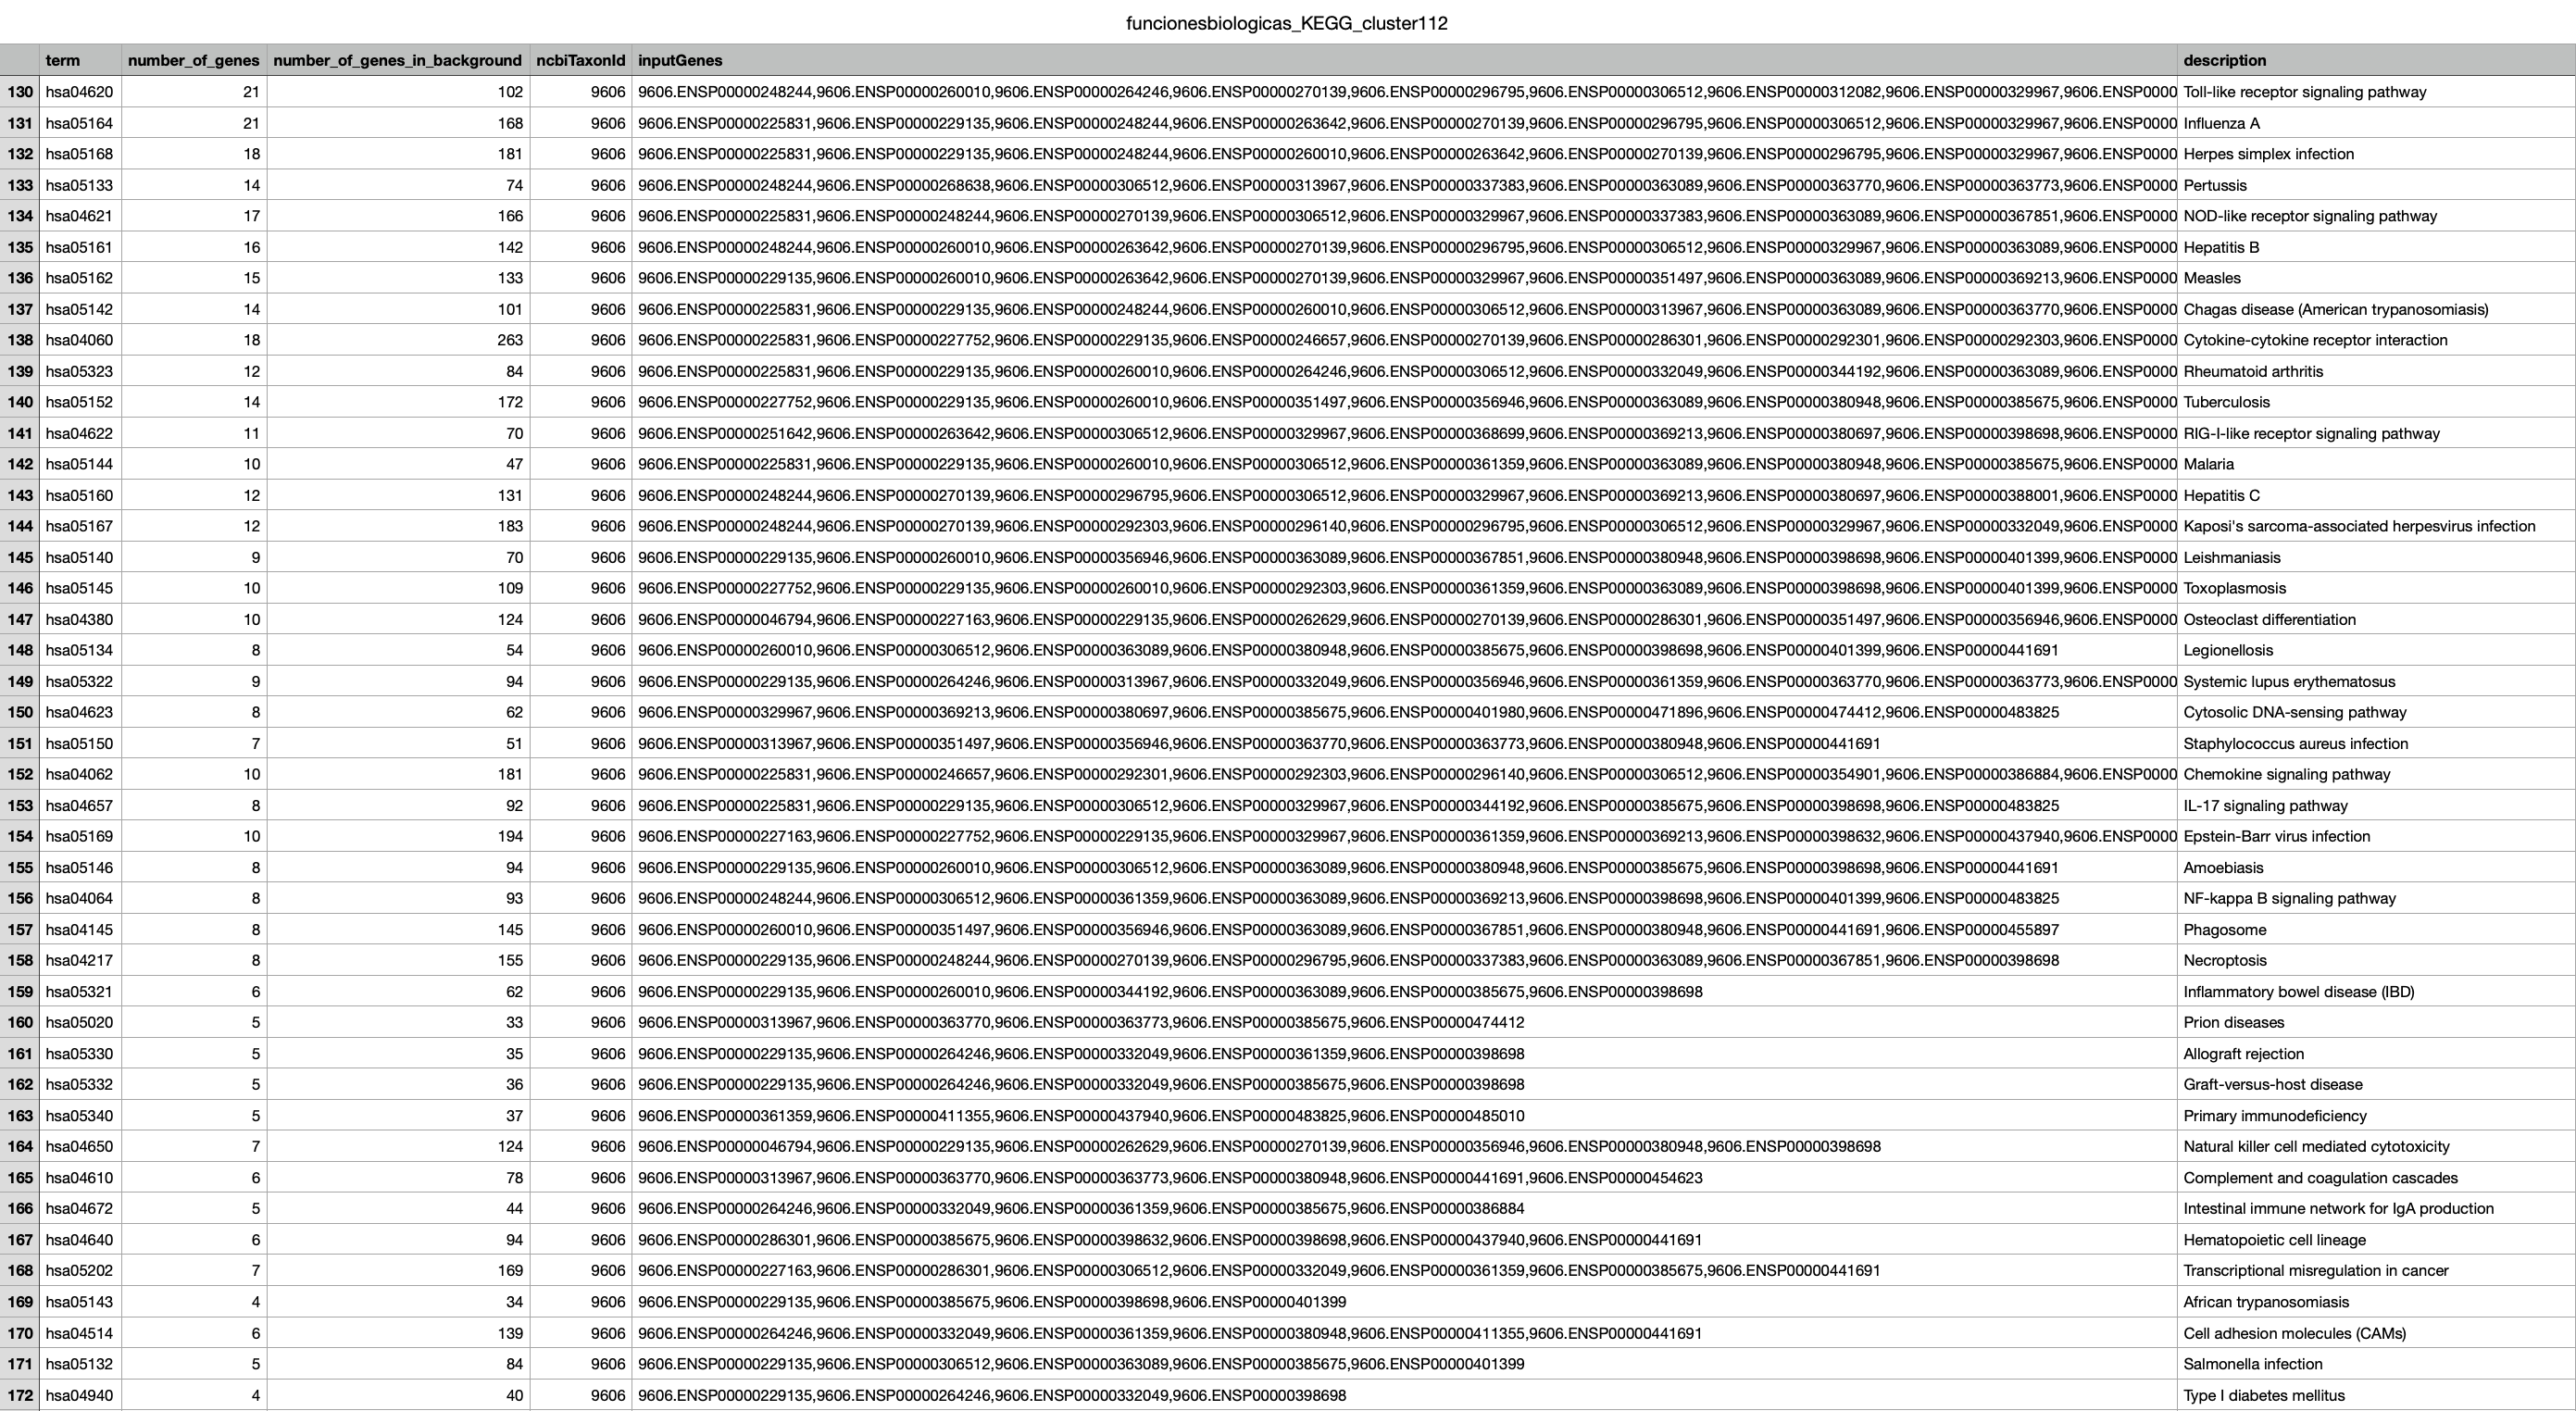
\includegraphics[width=70mm,scale=1.2]{figures/cluster112_KEGG.png}
	\caption{\textit{Funciones biológicas clúster 112 con KEGG}}
\end{figure}

Se puede observar que las funciones biológicas están relacionadas con enfermedades/infecciones (malaria, hepatitis B, tuberculosis) por lo que se podríamos deducir que dichas proteínas forman parte de la respuesta inmunitaria del organismo ante dichas enfermedades o que las provocan.
Además de esto, se observan funciones biológicas relacionadas con vías biológicas del organismo, como son la vía de señalización de quimioquinas, la de detección de ADN ctosólico...

\subsubsection{Clúster 78}

\paragraph{Enriquecimiento con GO}

\begin{figure}
	\centering
	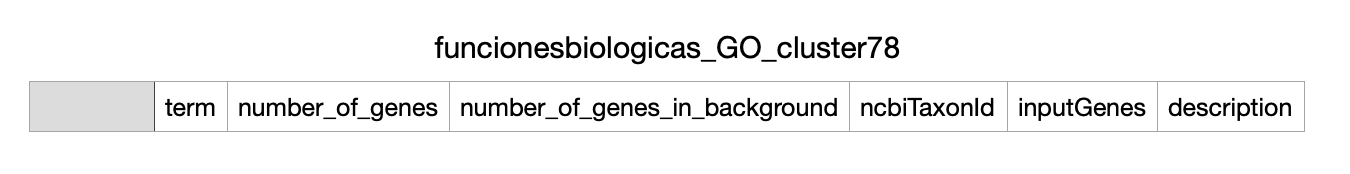
\includegraphics[width=70mm,scale=1.2]{figures/cluster78_GO.png}
	\caption{\textit{Funciones biológicas clúster 78 con GO}}
\end{figure}

En este resultado, GO no ha encontrado funciones biológicas asociadas al clúster elegido.

\paragraph{Enriquecimiento con KEGG}

\begin{figure}
	\centering
	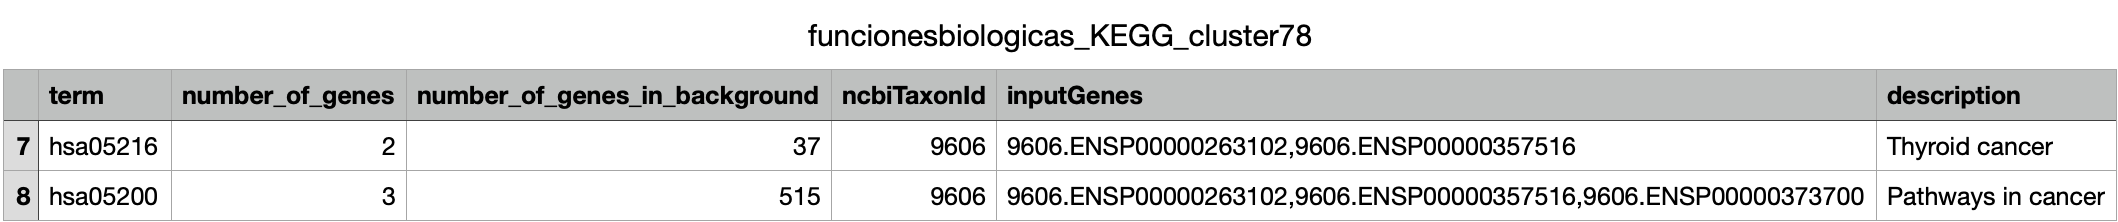
\includegraphics[width=70mm,scale=1.2]{figures/cluster78_KEGG.png}
	\caption{\textit{Funciones biológicas clúster 78 con KEGG}}
\end{figure}

En este caso, KEGG ha encontrado dos funciones biológicas asociadas al clúster: cáncer de tiroides y vías en el cáncer. Es por tanto que deducimos que las proteínas que forman parte de este clúster se ocupan de las vías principales del cáncer de tiroides, ya sea para detectarlo o provocarlo.

\subsubsection{Clúster 22}

\paragraph{Enriquecimiento con GO}

\begin{figure}
	\centering
	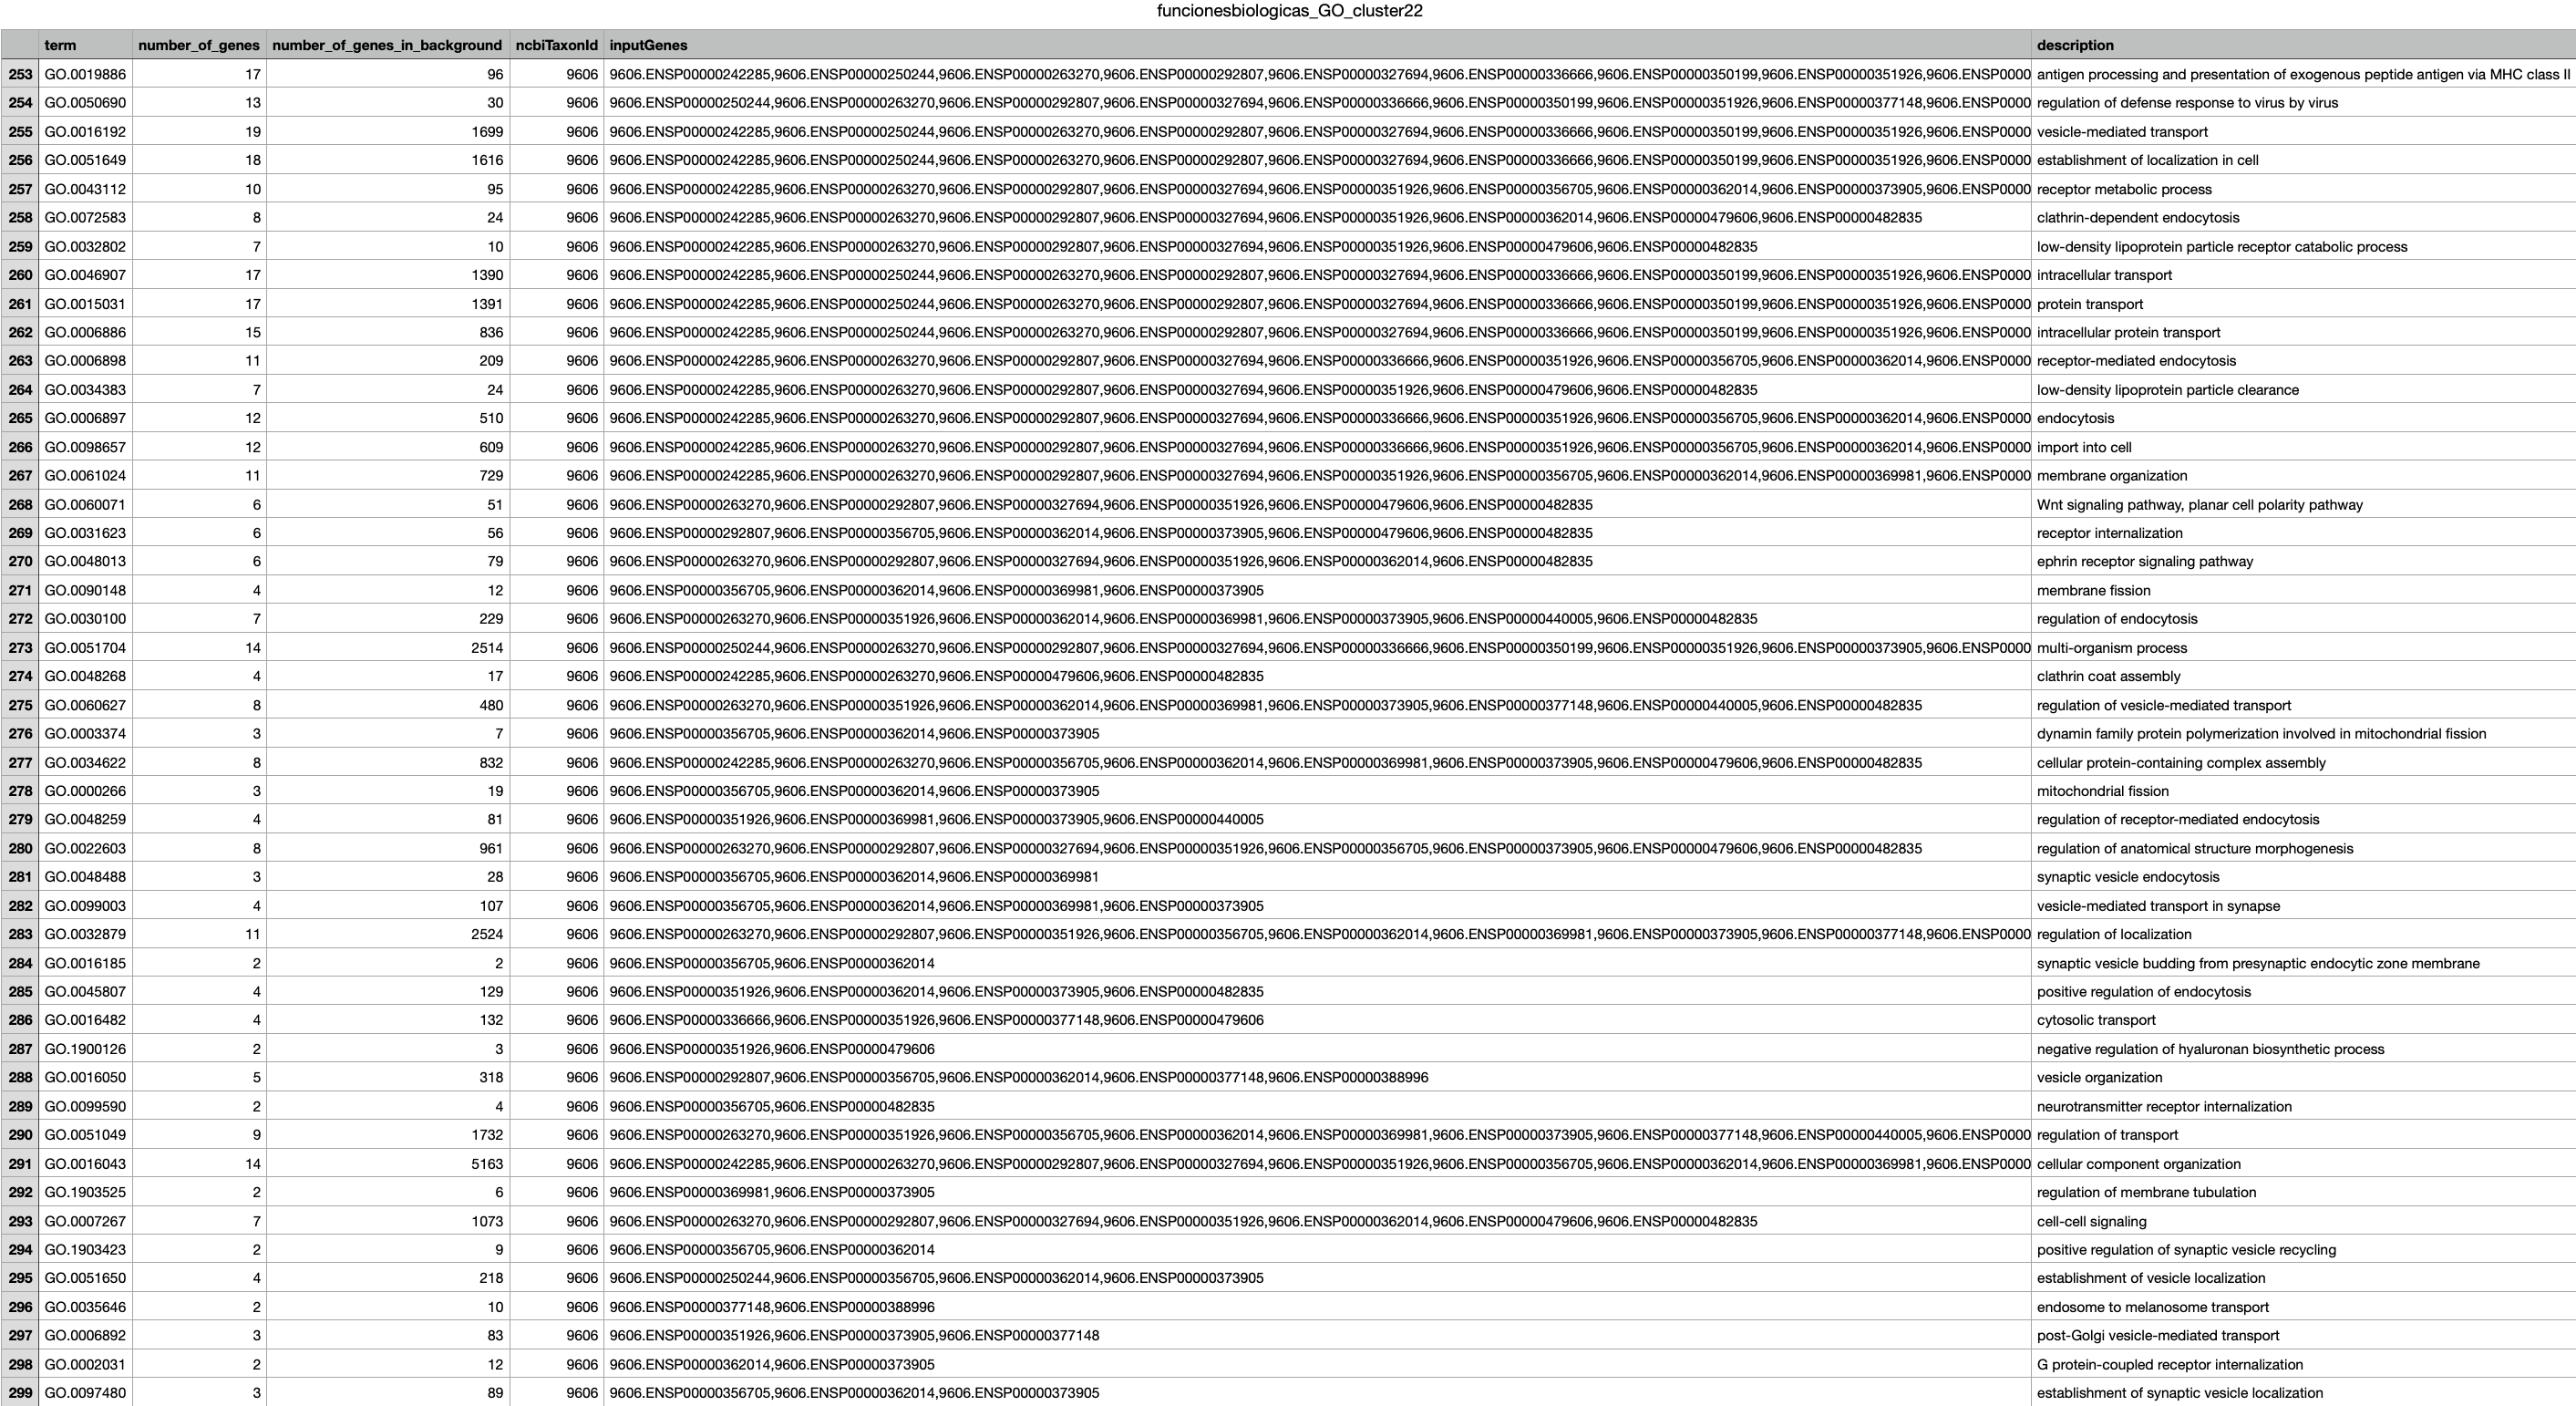
\includegraphics[width=70mm,scale=1.2]{figures/cluster22_GO.png}
	\caption{\textit{Funciones biológicas clúster 22 con GO}}
\end{figure}

En este caso, se puede observar que las principales funciones biológicas de las proteínas pertenecientes a este clúster son de regulación, transporte y recepción, por lo que desempeñan funciones muy importantes en las rutas metabólicas del organismo. 

\paragraph{Enriquecimiento con KEGG}

\begin{figure}
	\centering
	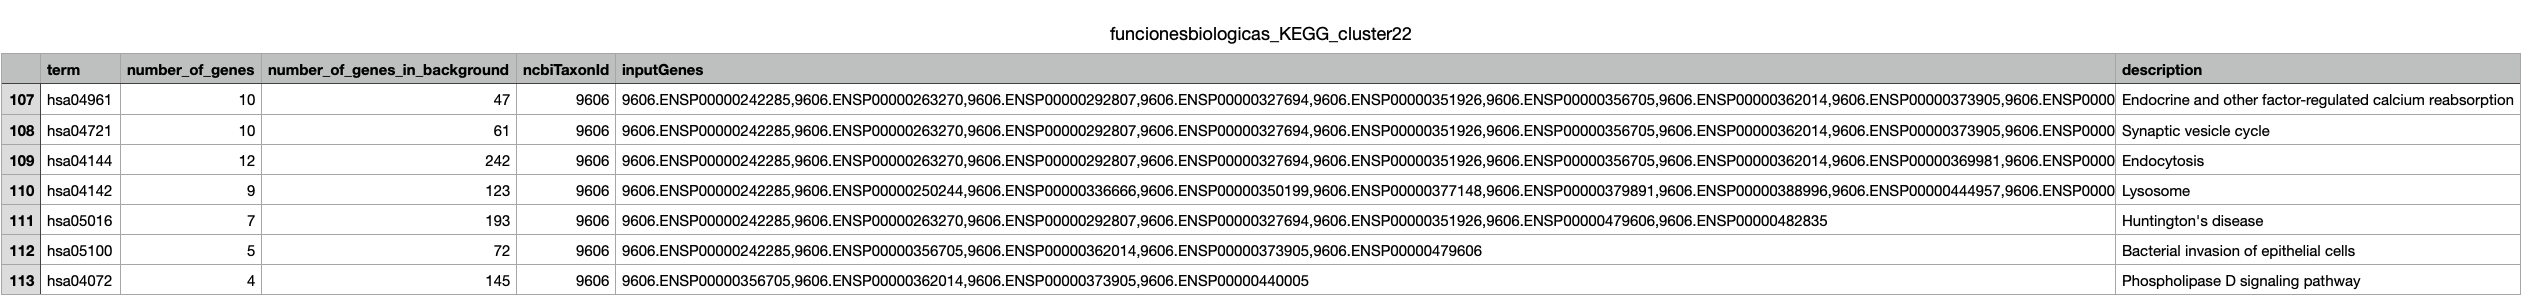
\includegraphics[width=70mm,scale=1.2]{figures/cluster22_KEGG.png}
	\caption{\textit{Funciones biológicas clúster 22 con KEGG}}
\end{figure}

Las funciones biológicas obtenidas por KEGG son más concretas: reabsorción de calcio regulada por factores endocrinos, ciclo de vesículas sinápticas, endocitosis, lisosoma, enfermedad de Huntington, invasión bacteriana de las células epiteliales y vía de señalización de la fosfolipasa D. Esta última está relacionada con la traducción de señales. Otras están relacionadas con enfermedades y sus causas.

\subsection{Clustering}



	\section{Discusión}

Una vez obtenidos los resultados, en este apartado se indagará en la relación que pueda tener el SarsCOV-2 con las funciones biológicas obtenidas previamente.

Tras el análisis funcional del \textbf{cluster 112}, descubrimos que una de las funciones con las que está muy relacionado es con el proceso metabólico de la fucosa. La fucosa es un azúcar que forma parte de algunas de las glucoproteínas que se encuentran en el aparato del Golgi cuando se produce la glucosilación.

Un estudio de Stanford Medicine (Estados Unidos) ha descubierto que aquellos pacientes que tenían una deficiencia en la fucosa, sufrían la enfermedad con más gravedad que los que tenían niveles normales. 
Además estos pacientes con leves niveles de fucosa, sus células inmunitarias presentaban niveles muy altos de unos receptores llamados CD16a, los cuales se sabe que aumentan la actividad inflamatoria de las células inmunitarias. 
Para una correcta respuesta inmunitaria es necesaria un poco de inflamación, sin embargo, si es demasiada puede producir que el paciente no tenga una respuesta inmunitaria buena y producir una  inflamación en los pulmones, lo que puede provocar que el paciente pueda llegar a un estado crítico. 

Así mismo, tras el análisis funcional del \textbf{cluster 22}, se ha llegado a la conclusión de que la principal función biológica que desempeñan las proteínas pertenecientes a dicho grupo afectan a la mitocondria de las células. El SarsCOV-2 secuestra las mitocondrias de las células inmunitarias, se replica dentro de las estructuras mitocondriales y altera la dinámica mitocondrial que conduce a la muerte celular, lo que aumenta la mortalidad de los pacientes que lo sufren.

De la misma forma, tras el análisis funcional del \textbf{cluster 78}, se ha llegado a la conclusión de que la principal función biológica que desempeñan las proteínas pertenecientes a dicho grupo afectan a la remodelación/degradación de la matriz extracelular de los pulmones. Los procesos patológicos que conducen a la disminución de la función pulmonar se usan para identificar mejor a los pacientes infectados con SARS-Co-V2 con mayor riesgo de deterioro agudo o daño fibrótico persistente del pulmón y, como consecuencia, se podría usar para guiar las decisiones de tratamiento.
	\section{Conclusiones}

Se ha llegado a la conclusión final de que las funciones biológicas de las proteínas estudiadas están basadas en el daño que el SarsCOV-2 le genera a los pulmones. 
Como se ha explicado, la fructosa los inflama y les genera un daño permanente que hace que las mitocondrias de las células se dañen y provoquen la muerte celular, lo que impide la regeneración de las matrices extracelulares de los pulmones.
Esto desencadenará en daños permanentes en los pacientes, lo que puede impedir su total recuperación, que se les desarrollen patologías crónicas o incluso que le provoquen la muerte (sepsis por COVID).
	
	
	%%%%%%%%%%%%%%%%%%%%%%%%%%%%%%%%%%%%%%%%%%%%%%
	%% OTRA INFORMACIÓN                         %%
	%%%%%%%%%%%%%%%%%%%%%%%%%%%%%%%%%%%%%%%%%%%%%%
	
	\begin{backmatter}
	
		\section*{Abreviaciones}%% if any
			
		
		\section*{Disponibilidad de datos y materiales}%% if any
			https://github.com/Paulandujar/project\_template
		
		\section*{Contribución de los autores}
<<<<<<< Updated upstream
			I.R.G: Encargada del análisis de la red (distancia entre nodos, distribución de grado y coeficiente de agrupamiento), cálculo de la robustez, escritura del launch.sh y escritura de los resultados de estos cálculos en el report; P.A.Z: Encargada del cálculo linked communities, posterior análisis de esos resultados en el report y escritora del abstract; R.G.M: Encargada de las funciones de Robustez y escritura del apartado Materiales y Métodos; S.dC.C: Encargada del enriquecimiento funcional, análisis de esos resultados en el report y escritura del setup.sh 
=======
		
			I.R.G: Encargada del análisis de la red (distancia entre nodos, distribución de grado y coeficiente de agrupamiento), cálculo de la robustez, escritura del launch.sh y escritura de los resultados de estos cálculos en el report; P.A.Z: Encargada del cálculo linked communities, posterior análisis de esos resultados en el report y escritora del abstract; R.G.M: Encargada de las funciones de Robustez y escritura del apartado Materiales y Métodos; S.dC.C: Encargada del enriquecimiento funcional, análisis de esos resultados en el report y escritura del setup.sh
		
>>>>>>> Stashed changes
		
		
		%%%%%%%%%%%%%%%%%%%%%%%%%%%%%%%%%%%%%%%%%%%%%%%%%%%%%%%%%%%%%%%%%%%%%%%%%%%%%%%%%%%%%%%%
		%% BIBLIOGRAFIA: no teneis que tocar nada, solo sustituir el archivo bibliography.bib %%
		%% por el que hayais generado vosotros                                                %%
		%%%%%%%%%%%%%%%%%%%%%%%%%%%%%%%%%%%%%%%%%%%%%%%%%%%%%%%%%%%%%%%%%%%%%%%%%%%%%%%%%%%%%%%%
		
		\bibliographystyle{bmc-mathphys} % Style BST file (bmc-mathphys, vancouver, spbasic).
		\bibliography{bibliography}      % Bibliography file (usually '*.bib' )
	
	\end{backmatter}
\end{document}
